%%%%%%%%%%%%%%%%%%%%%%%%%%%%%%%%%%%%%%%%%%%%%%%%%%%%%%%%%%%%%%%%%%%
%
% Ce gabarit peu servir autant les philosophes que les scientifiques ; 
% et même d'autres genres, vous en faites ce que vous voulez.
% J'ai modifié et partagé ce gabarit afin d'épargner à d'autres 
% d'interminables heures à modifier des gabarits d'articles anglais. 
% 
% L'ajout d'une table des matières et une bibliographie a été ajoutée,
% rendant le gabarit plus ajusté aux besoins de plusieurs.
%
% Pour retrouvé le gabarit original, veuillez télécharger les
% documents suivants: llncs2e.zip (.cls et autres) et 
% typeinst.zip (.tex). Les documents ci-haut mentionnés ne sont pas 
% disponibles au même endroit, alors je vous invite à fouiller le web. 
%
% Pour l'instant (02-2016) ils sont disponibles tous deux ici :
%
% http://kawahara.ca/springer-lncs-latex-template/
%
% Netkompt
%
%%%%%%%%%%%%%%%%%%%%%%%%%%%%%%%%%%%%%%%%%%%%%%%%%%%%%%%%%%%%%%%%%%%


%%%%%%%%%%%%%%%%%%%%%%% file typeinst.tex %%%%%%%%%%%%%%%%%%%%%%%%%
%
% This is the LaTeX source for the instructions to authors using
% the LaTeX document class 'llncs.cls' for contributions to
% the Lecture Notes in Computer Sciences series.
% http://www.springer.com/lncs       Springer Heidelberg 2006/05/04
%
% It may be used as a template for your own input - copy it
% to a new file with a new name and use it as the basis
% for your article.
%
% NB: the document class 'llncs' has its own and detailed documentation, see
% ftp://ftp.springer.de/data/pubftp/pub/tex/latex/llncs/latex2e/llncsdoc.pdf
%
%%%%%%%%%%%%%%%%%%%%%%%%%%%%%%%%%%%%%%%%%%%%%%%%%%%%%%%%%%%%%%%%%%%

\documentclass[runningheads,a4paper]{llncs}

\usepackage[utf8]{inputenc}

\usepackage{natbib}
\bibliographystyle{apalike-fr}

\usepackage{amssymb}
\setcounter{tocdepth}{3}
\usepackage{graphicx}

\usepackage[french]{babel} % Pour adopter les règles de typographie française
\usepackage[T1]{fontenc} % Pour que les lettres accentuées soient reconnues

\usepackage{url}
\urldef{\mailsa}\path|{alfred.hofmann, ursula.barth, ingrid.haas, frank.holzwarth,|
\urldef{\mailsb}\path|anna.kramer, leonie.kunz, christine.reiss, nicole.sator,|
\urldef{\mailsc}\path|erika.siebert-cole, peter.strasser, lncs}@springer.com|    
\newcommand{\keywords}[1]{\par\addvspace\baselineskip
\noindent\keywordname\enspace\ignorespaces#1}

\begin{document}

\mainmatter 

\title{Gabarit : article français}

\titlerunning{Gabarit : article français}

\author{Nom de l'auteur}

\institute{Nom de l'institution}

\authorrunning{Nom de l'auteur}

\toctitle{Résumé}
\tocauthor{{}}

\maketitle

\begin{abstract}
Ici va le résumé
\end{abstract}

\medskip

\begingroup
\let\clearpage\relax
\tableofcontents
\addcontentsline{toc}{section}{Introduction}
\endgroup

\medskip
\medskip

\section*{Introduction}

Vous trouverez des informations pertinentes concernant ce gabarit (en anglais)
dans le reste de ce document.

The \LaTeX{} source of this instruction file for \LaTeX{} users may be
used as a template. This is
located in the ``authors'' subdirectory in
\url{ftp://ftp.springer.de/pub/tex/latex/llncs/latex2e/instruct/} and
entitled \texttt{typeinst.tex}. There is a separate package for Word 
users. Kindly send the final and checked source
and PDF files of your paper to the Contact Volume Editor. This is
usually one of the organizers of the conference. You should make sure
that the \LaTeX{} and the PDF files are identical and correct and that
only one version of your paper is sent. It is not possible to update
files at a later stage. Please note that we do not need the printed
paper.

\section{Première section}

Vous trouverez des informations pertinentes concernant ce gabarit (en anglais)
dans le reste de ce document.

The \LaTeX{} source of this instruction file for \LaTeX{} users may be
used as a template. This is
located in the ``authors'' subdirectory in
\url{ftp://ftp.springer.de/pub/tex/latex/llncs/latex2e/instruct/} and
entitled \texttt{typeinst.tex}. There is a separate package for Word 
users. Kindly send the final and checked source
and PDF files of your paper to the Contact Volume Editor. This is
usually one of the organizers of the conference. You should make sure
that the \LaTeX{} and the PDF files are identical and correct and that
only one version of your paper is sent. It is not possible to update
files at a later stage. Please note that we do not need the printed
paper.

\subsubsection{Headings.}

Headings should be capitalized
(i.e., nouns, verbs, and all other words
except articles, prepositions, and conjunctions should be set with an
initial capital) and should,
with the exception of the title, be aligned to the left.
Words joined by a hyphen are subject to a special rule. If the first
word can stand alone, the second word should be capitalized.

Here are some examples of headings: ``Criteria to Disprove
Context-Freeness of Collage Language", ``On Correcting the Intrusion of
Tracing Non-deterministic Programs by Software", ``A User-Friendly and
Extendable Data Distribution System", ``Multi-flip Networks:
Parallelizing GenSAT", ``Self-determinations of Man".

\subsubsection{Lemmas, Propositions, and Theorems.}

The numbers accorded to lemmas, propositions, and theorems, etc. should
appear in consecutive order, starting with Lemma 1, and not, for
example, with Lemma 11.

\subsection{Figures}

For \LaTeX\ users, we recommend using the \emph{graphics} or \emph{graphicx}
package and the \verb+\includegraphics+ command.

Please check that the lines in line drawings are not
interrupted and are of a constant width. Grids and details within the
figures must be clearly legible and may not be written one on top of
the other. Line drawings should have a resolution of at least 800 dpi
(preferably 1200 dpi). The lettering in figures should have a height of
2~mm (10-point type). Figures should be numbered and should have a
caption which should always be positioned \emph{under} the figures, in
contrast to the caption belonging to a table, which should always appear
\emph{above} the table; this is simply achieved as matter of sequence in
your source.

Please center the figures or your tabular material by using the \verb+\centering+
declaration. Short captions are centered by default between the margins
and typeset in 9-point type (Fig.~\ref{fig:example} shows an example).
The distance between text and figure is preset to be about 8~mm, the
distance between figure and caption about 6~mm.

To ensure that the reproduction of your illustrations is of a reasonable
quality, we advise against the use of shading. The contrast should be as
pronounced as possible.

If screenshots are necessary, please make sure that you are happy with
the print quality before you send the files.
\begin{figure}
\centering
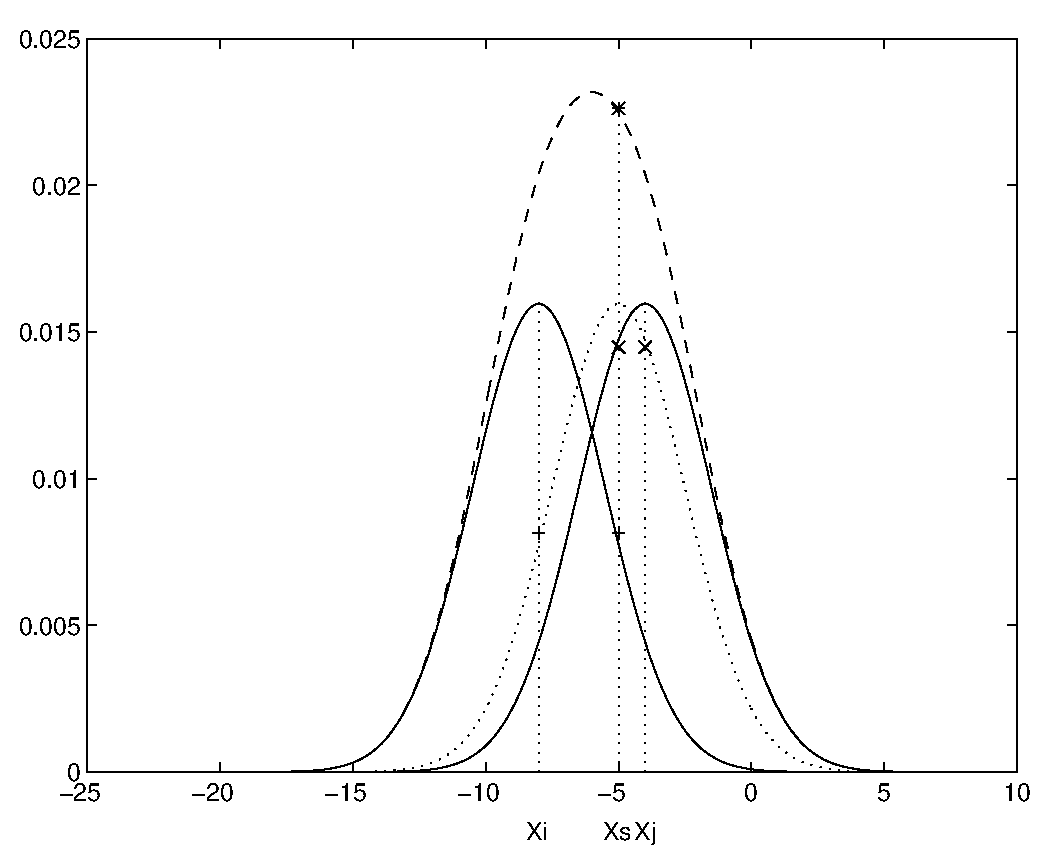
\includegraphics[height=6.2cm]{eijkel2}
\caption{One kernel at $x_s$ (\emph{dotted kernel}) or two kernels at
$x_i$ and $x_j$ (\textit{left and right}) lead to the same summed estimate
at $x_s$. This shows a figure consisting of different types of
lines. Elements of the figure described in the caption should be set in
italics, in parentheses, as shown in this sample caption.}
\label{fig:example}
\end{figure}

Please define figures (and tables) as floating objects. Please avoid
using optional location parameters like ``\verb+[h]+" for ``here".

\paragraph{Remark 1.}

In the printed volumes, illustrations are generally black and white
(halftones), and only in exceptional cases, and if the author is
prepared to cover the extra cost for color reproduction, are colored
pictures accepted. Colored pictures are welcome in the electronic
version free of charge. If you send colored figures that are to be
printed in black and white, please make sure that they really are
legible in black and white. Some colors as well as the contrast of
converted colors show up very poorly when printed in black and white.

\subsection{Formulas}

Displayed equations or formulas are centered and set on a separate
line (with an extra line or halfline space above and below). Displayed
expressions should be numbered for reference. The numbers should be
consecutive within each section or within the contribution,
with numbers enclosed in parentheses and set on the right margin --
which is the default if you use the \emph{equation} environment, e.g.,
\begin{equation}
  \psi (u) = \int_{o}^{T} \left[\frac{1}{2}
  \left(\Lambda_{o}^{-1} u,u\right) + N^{\ast} (-u)\right] dt \;  .
\end{equation}

Equations should be punctuated in the same way as ordinary
text but with a small space before the end punctuation mark.

\subsection{Footnotes}

The superscript numeral used to refer to a footnote appears in the text
either directly after the word to be discussed or -- in relation to a
phrase or a sentence -- following the punctuation sign (comma,
semicolon, or period). Footnotes should appear at the bottom of
the
normal text area, with a line of about 2~cm set
immediately above them.\footnote{The footnote numeral is set flush left
and the text follows with the usual word spacing.}

\subsection{Program Code}

Program listings or program commands in the text are normally set in
typewriter font, e.g., CMTT10 or Courier.

\section{Deuxième section}

\subsection{ainsi de suite...}

\medskip

\noindent
{\it Example of a Computer Program}
\begin{verbatim}
program Inflation (Output)
  {Assuming annual inflation rates of 7%, 8%, and 10%,...
   years};
   const
     MaxYears = 10;
   var
     Year: 0..MaxYears;
     Factor1, Factor2, Factor3: Real;
   begin
     Year := 0;
     Factor1 := 1.0; Factor2 := 1.0; Factor3 := 1.0;
     WriteLn('Year  7% 8% 10%'); WriteLn;
     repeat
       Year := Year + 1;
       Factor1 := Factor1 * 1.07;
       Factor2 := Factor2 * 1.08;
       Factor3 := Factor3 * 1.10;
       WriteLn(Year:5,Factor1:7:3,Factor2:7:3,Factor3:7:3)
     until Year = MaxYears
end.
\end{verbatim}
%
\noindent
{\small (Example from Jensen K., Wirth N. (1991) Pascal user manual and
report. Springer, New York)}

\bibliography{references}
\nocite{*} 

\end{document}
